\documentclass[UTF8,a4paperdui, % draft
]{ctexart}
\usepackage[hidelinks]{hyperref}
\usepackage{bm}
\usepackage{graphicx}
\usepackage{pdfpages}
\usepackage{amsmath}
\usepackage{cite}
\usepackage{caption,subcaption}
\usepackage{geometry}
\usepackage{pdfpages}
\usepackage[ruled,vlined,boxed,linesnumbered]{algorithm2e}
\usepackage{fontspec}
\setmainfont{Times New Roman}
\setmonofont{Consolas}
\usepackage{listings}
\usepackage{color}
\definecolor{eclipseBlue}{RGB}{42,0.0,255}
\definecolor{eclipseGreen}{RGB}{63,127,95}

\lstset {
  basicstyle=\small\ttfamily,
  captionpos=b,
  tabsize=2,
  columns=fixed,
  breaklines=true,
  frame=l,
  numbers=left,
  numberstyle=\small\ttfamily,
  morekeywords= {
    EQUAL, GREATER, LESS, NONE, SOME, abstraction, abstype, and, andalso, array, as, before, bool, case, char, datatype, do, else, end, eqtype, exception, exn, false, fn, fun, functor, handle, if, in, include, infix, infixr, int, let, list, local, nil, nonfix, not, o, of, op, open, option, orelse, overload, print, raise, real, rec, ref, sharing, sig, signature, string, struct, structure, substring, then, true, type, unit, val, vector, where, while, with, withtype, word
  },
  morestring=[b]",
  morecomment=[s]{(*}{*)},
  stringstyle=\color{black},
  identifierstyle=\color{eclipseBlue},
  keywordstyle=\color{red},
  commentstyle=\color{eclipseGreen}
}
\graphicspath{{Figures/}}%文章所用图片在当前目录下的 Figures目录
\geometry{left=4.0cm,right=4.0cm,top=5cm,bottom=5cm}
%%%%%%%%%%%%%%%%%%%%%%%%%%%%
%%%%%%%%%%%%%%%%%%%%%%%%%%%%
\DeclareMathOperator{\net}{net}
\DeclareMathOperator{\sups}{SuperString}
%%%%%%%%%%%%%%%%%%%%%%%%%%%%
%%%%%%%%%%%%%%%%%%%%%%%%%%%%

\makeatletter
\algocf@newcmdside@kobe{LetIn@let}{%
\KwSty{let}%
\ifArgumentEmpty{#1}\relax{ #1}%
\algocf@group{#2}%
\par
}
\algocf@newcmdside@kobe{LetIn@in}{%
\KwSty{in}%
\ifArgumentEmpty{#1}\relax{ #1}%
\algocf@block{#2}{end}{#3}%
\par
}
\newcommand\LetIn[2]{%
\LetIn@let{#1}%
\LetIn@in{#2}%
}
\makeatother

\newcommand\op{\texttt{op}}
\newcommand\ttt{\texttt}
\newcommand\tbf{\textbf}
\newcommand\tit{\textit}
\newcommand\tttt[1]{\text{\ttt{#1}}}
\newcommand\givepar[2]{\ttt{)}$^{#1\ #2}$\ttt{(}}
\usepackage{amssymb}
\usepackage{extarrows}
\begin{document}
\newpage
\newcommand*{\calF}{\mathcal{F}}
\newcommand*{\calH}{\mathcal{H}}
\newcommand*{\vx}{\bm x}
\newcommand*{\vy}{\bm y}
\newcommand*{\vh}{\bm h}
\newcommand{\Figure}[2]{
\begin{figure}[htbp]
\centering
\includegraphics[height=#1]{#2}
\end{figure}
}
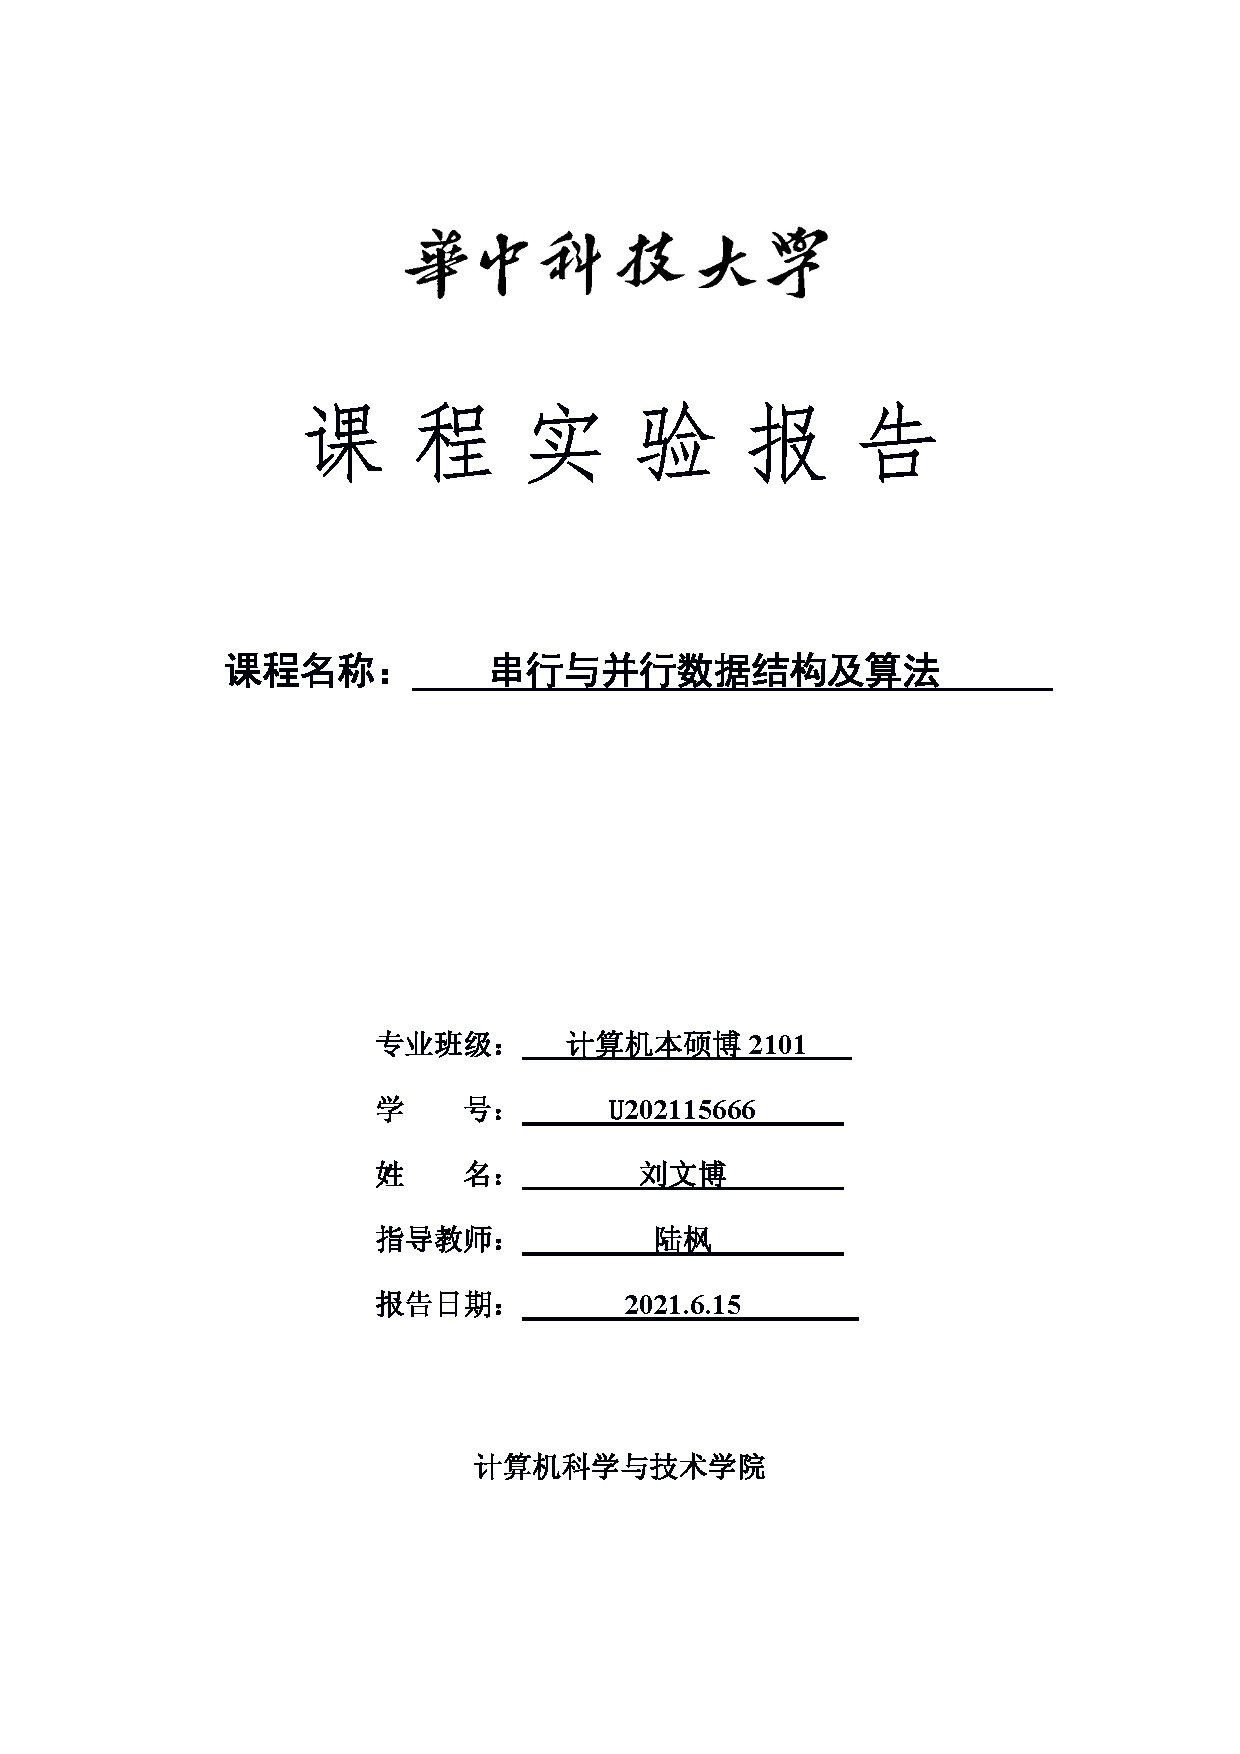
\includepdf{cover}
\setcounter{tocdepth}{1}
\tableofcontents

\newpage
\section{实验一:无重复排序}

\subsection{题目描述}
给出一个具有$ N $个互不相同元素的数组,请对它进行升序排序。第一行为一个整数 N,
表示元素的个数。第二行为$ N $个整数,表示这$ N $个元素,保证每个元素均在 int 范围内

\subsection{算法流程}
本题使用快速排序,做法是用$sml$的$List.partition$函数将序列分为小于$x$和大于$x$的两部分,进行递归求解,然后将两个子序列连接得到原问题的解。
\par 由于$partition$本身就做了比较操作,故递归边界是子问题规模为0时返回一个空序列。

\begin{lstlisting}
    val N = getInt();
    val a = getIntTable(N);
    fun quickSort [] = []
    | quickSort(x::xs) =
    let val (left, right) = List.partition(fn y => y < x) xs
    in
    quickSort(left) @ [x] @ quickSort(right) end
    val res = quickSort(a);
    printIntTable(res);
\end{lstlisting}

\subsection{复杂度分析}
$partition$的$Work$为$O(n)$,$Span$为$O(lgn)$,我们每次选择序列的第一个元素为pivot。
\par 最好情况下每次都能将序列划分为相等的两部分
$$W(n)=2W(\frac{n}{2})+O(n)$$
$$S(n)=2S(\frac{n}{2})+S(lgn)$$
\par 由主定理$W(n)=O(nlgn),S(n)=O({lg}^2n)$

\par 最坏情况下序列基本有序,总是将序列划分为一个大小为n-1的子序列和一个空序列
$$W(n)=W(n-1)+O(n)$$
$$S(n)=S(n-1)+S(lgn)$$
\par 由主定理$W(n)=O(n^2),S(n)=O(nlgn)$
\\\
\par  在平均情况下,假设输入数组的元素是随机分布的,选择第一个元素作为枢轴的快速排序的平均复杂度分析为$W(n)=O(nlgn),S(n)=O({lg}^2n)$

\subsection{样例分析}
测试样例如下图所示,它是一个长度为10的序列
\Figure{0.075\textheight}{example1.png}\\
首先选择 10 作为基准元素,进行划分得到[[9 6] 10 [155 200 60 174 17 172 103]]\\
\\\
然后对于左边和右边的再次进行同样的步骤,左边以 9作为基准元素,右边以 155 作为基准元素,进行划分得到[[6] 9 []] [[60 17 103] 155 [200 174 172]]\\
\\\
继续这样不断递归,直到子序列长度为 0 时终止递归,返回结果,按照左边 + 基准元素 + 右边 的方式将其连接并返回\\
\\\
最终返回结果[6,9,10,17,60,103,155,172,174,200]

\newpage
\section{实验二:最短路}

\subsection{题目描述}
给定一个带权无向图,一个源点,权值在边上。计算从源点到其他各点的最短路径。
输入格式为:
\begin{itemize}
    \item 第一行:3个由空格隔开的整数: $N, M, T_s$ 。其中 $N$ 表示结点的数量(从1到 $N$ ), $M$ 表示边的 数量, $T_s$ 表示源点
    \item  第 2 到第 $M+1$ 行:描述每条边,每行包含 3 个由空格隔开的整数: $R_s, R_e, C_i$ ,其中 $R_s$ 和 $R_e$ 是两个结点的编号, $C_i$ 是它们之间的边的权值
\end{itemize}
输出格式为:
\begin{itemize}
    \item $N$个整数,表示从源点$T_s$到各顶点的最短路径长度。如果到某个顶点不连通,对应最短路径长度输出 -1。
\end{itemize}
\subsection{算法流程}
本题需要计算从源点到其他各点的最短路径,因为不存在路径长度为负的情况,可以使用 Dijkstra 算法来解决\\
算法描述如下:
\begin{enumerate}
    \item 创建一个初始值足够大的长度为$N$的数组$distance[]$来记录记录源点到所有点的最短距离
    \item 创建一个初始值为false的长度为$N$的布尔数组$visited[]$来记录该点是否已被访问
    \item 在未访问的顶点中,找到距离源点最近的顶点,将其标记为已访问
    \item 更新与该顶点相邻的未访问顶点的最短路径长度,如果经过当前顶点到达相邻顶点的路径长度比原先的路径长度短,则更新最短路径长度
    \item 如果还有节点没有访问,回到步骤3
    \item 此时$distance[]$中的值即为源点到各顶点的最短路径长度,输出该值
\end{enumerate}
算法伪代码描述如下:\\
function Dijkstra(graph, source):\\
distance[source] $=0$\\
for $i=1$ to $N$ :\\
  if $i \neq$ source:\\
    distance $[i]=$ $\infty$\\
visited[source] = true\\
for $k=1$ to $\mathrm{N}-1$ :\\
  minDist $=$ $\infty$\\
  $u=-1$\\
  for $v=1$ to $\mathrm{N}$ :\\
    if visited $[v]=$ false and $\operatorname{distance}[v]$ $<$ minDist:\\
      $\operatorname{minDist}=\operatorname{distance}[v]$\\
      $\mathrm{u}=\mathrm{v}$\\
  if $u=-1$ :\\
    break\\
  visited $[u]=$ true\\
  for $v=1$ to $\mathrm{N}$ :\\
    if visited $[v]=$ false and $\operatorname{graph}[u][v]>0$ :\\
      if distance[u] $+\operatorname{graph}[u][v]<\operatorname{distance}[v]$ :\\
         $\operatorname{distance}[v]=\operatorname{distance}[u]+\operatorname{graph}[u][v]$\\
return distance
\subsection{复杂度分析}
步骤三在未访问的顶点中,找到距离源点最近的顶点需要$O(n)$的$Work$和$O(lgn)$的$Span$\\
步骤四更新与该顶点相邻的未访问顶点的最短路径长度需要$O(n)$的$Work$和$O(1)$的$Span$\\
$Dijkstra$是一个典型的串行算法,它的每次计算都依赖前面的结果\\
那么总的$Work$为$O(n^2)$,$Span$为$O(nlgn)$\\\
用邻接矩阵保存图,用两个长度为N的数组来记录距离和标记访问,则总的空间复杂度为$O(n^2)$
\subsection{样例分析}
测试样例如下图所示,它是一个包含7个节点,15条边的图,其中源点为5号节点
\Figure{0.3\textheight}{example2.png}\\
算法过程如下:
\begin{enumerate}
    \item $distance$为$[\infty,\infty,\infty,\infty,\textcolor{red}{0},\infty,\infty]$
    \item $visited$为$[false,false,false,false,\textcolor{red}{true},false,false]$
    \item minDist为未访问的6号节点到源点的距离3,更新$distance$为$[\infty,\infty,\infty,\infty,0,\textcolor{red}{3},\infty]$,$visited$为$[false,false,false,false,true,\textcolor{red}{true},false]$
    \item 更新与6号节点相邻的未访问顶点的最短路径长度,更新$distance$为$[\textcolor{red}{4},\infty,\textcolor{red}{7},\infty,0,3,\infty]$
    \item 还有节点未访问,minDist为未访问的1号节点到源点的距离4,更新$visited$为$[\textcolor{red}{true},false,false,false,true,true,false]$
    \item 更新与1号节点相邻的未访问顶点的最短路径长度,更新$distance$为$[4,\infty,7,\textcolor{red}{7},0,3,\infty]$
    \item 还有节点未访问,minDist为未访问的7号节点到源点的距离5,更新$distance$为$[4,\infty,7,7,0,3,\textcolor{red}{5}]$,$visited$为$[true,false,false,false,true,true,\textcolor{red}{true}]$
    \item 更新与7号节点相邻的未访问顶点的最短路径长度,更新$distance$为$[4,\textcolor{red}{6},7,7,0,3,5]$
    \item 还有节点未访问,minDist为未访问的2号节点到源点的距离6,更新$visited$为$[true,\textcolor{red}{true},false,false,true,true,false]$
    \item 更新与4号节点相邻的未访问顶点的最短路径长度,$distance$不变,此时我们其实已经得到了最终答案
    \item 重复上面的过程,直到所有节点都被访问
    \item 此时$distance[]$中的值即为源点到各顶点的最短路径长度,输出$[4,6,7,7,0,3,5]$
\end{enumerate}

\newpage
\section{实验三:最大括号距离}

\subsection{题目描述}
现在给你一个串,你需要找出所有这个串中匹配的子串(一个闭合的串,并且外侧由括号包裹)中最长
的那个,输出它的长度。第一行输入一个数N,表示序列的长度,满足N≤30000。 接下来一行输入N个
数,表示这个括号序列,0代表左括号,1代表右括号。

\subsection{算法流程}
我们可以用栈来解决该问题,遍历括号序列,当遇到左括号时,将其位置入栈;当遇到右括号时,从栈顶去除相对应的左括号的位置,计算括号的距离(右括号减左括号加1),并更新最大距离。最后返回最大距离即可\\
\\\
实现代码如下
\begin{lstlisting}
 (*****Begin*****)			 
val N = getInt();   
val s = ListPair.zip(List.tabulate(N, fn x => x),getIntTable(N));
fun parenDist((pos, x), (stack, max)) =
    if x = 0 then (pos::stack, max) 
    else if stack = [] then (stack, max)
    else
        let val top = hd stack
        val tmp = Int.max(max, pos - top + 1)
        in
        (tl stack, tmp) end; 
val res = #2(foldl parenDist ([], 0) s);
printInt(res);
(*****End*****)
\end{lstlisting}
其中pos记录括号的位置,x是当前读到的括号序列的值,stack是一个序列用来实现栈
\subsection{复杂度分析}
该算法遍历输入序列,故其$Work=Span=O(n)$,使用栈来模式匹配,空间复杂度为$O(n)$
\subsection{样例分析}
测试样例如下图所示,它是一个长度为10的序列
\Figure{0.1\textheight}{example3.png}\\
算法过程如下:
\begin{enumerate}
    \item 栈为空,max=0
    \item 第零个元素是0,pos=0入栈
    \item 第一个元素是0,pos=1入栈
    \item 第二个元素是1,出栈并计算当前括号的距离为2-1+1=2,更新max=2
    \item 第三个元素是0,pos=3入栈
    \item 第四个元素是1,出栈并计算当前括号的距离为4-3+1=2
    \item 第五个元素是1,出栈并计算当前括号的距离为5-0+1=6,更新max=2
    \item 第六个元素是0,pos=6入栈
    \item 第七个元素是0,pos=7入栈
    \item 第八个元素是1,出栈并计算当前括号的距离为8-7+1=2
    \item 第九个元素是1,出栈并计算当前括号的距离为9-6+1=4
    \item 得到max=6
\end{enumerate}

\newpage
\section{实验四:天际线}
\subsection{题目描述}
第一行输入一个整数$N$,表示建筑的数量 。接下来N行 , 每行输入3个整数$li ,hi ,ri$ 分别为建筑的左边界坐标,高度,右边界坐标\\
输出天际线的轮廓,即在建筑高度发生突变的位置输出建筑坐标以及建筑的高度(在建筑重合的地方我们可以知道低的建筑可以被高的建筑阻挡,因此我
们只需注意每个坐标的最高建筑的高度即可)

\subsection{算法流程}
采用扫描线的算法,只在边界点进行比较,使用优先队列维护最大高度,使用一个轮廓列表来存储轮廓结果
\begin{enumerate}
    \item 在输入数据的基础上加入地平线
    \item 使用快速排序按左边界坐标对输入的建筑物进行排序
    \item 对所有边界点进行快排
    \item 遍历排序后的边界点序列,将左边界等于当前边界点的建筑的高度入队,将右边界等于当前边界点的建筑的高度出队,当最大高度(优先队列队首元素)改变时将当前坐标和新的最大高度存入轮廓列表
    \item 输出轮廓序列
\end{enumerate}

\subsection{复杂度分析}
步骤一的快速排序的$Work$为$O(nlgn)$,$Span$为$O(lg^2n)$\\
步骤二串行扫描,每次更新需要保持优先队列有序,则$Work=Span=O(lgn)$,一共2n次,所以$Work=Span=O(nlgn)$\par
故算法总的$Work=Span=O(nlgn)$\par
算法的空间复杂度易知为$O(n)$

\subsection{样例分析}
测试样例如下图所示,它包含4个建筑物
\Figure{0.25\textheight}{example4.png}\\
算法过程如下:
\begin{enumerate}
    \item 边界点序列为$[1,3,4,6,7,8,10,11]$,同时得到有序的建筑物序列
    \item 当前边界点为1,地平线(1,0,11)和(1,3,4)入队,队首元素为(1,3,4),(1,3)存入轮廓序列
    \item 当前边界点为3,(3,2,11)入队
    \item 当前边界点为4,(1,3,4)出队,队首元素为(3,2,11),(4,2)存入轮廓序列
    \item 当前边界点为6,(6,6,8)入队,队首元素为(6,6,8),(6,6)存入轮廓序列
    \item 当前边界点为7,(7,4,10)入队
    \item 当前边界点为8,(6,6,8)出队,队首元素为(7,4,10),(8,4)存入轮廓序列
    \item 当前边界点为10,(7,4,10)出队,队首元素为(3,2,11),(10,2)存入轮廓序列
    \item 当前边界点为11,(3,2,11)出队,队首元素为(1,0,11),(11,0)存入轮廓序列
    \item 输出轮廓序列
\end{enumerate}

\newpage
\section{实验五:括号匹配}

\subsection{题目描述}
给定一个括号序列,判断它是否是匹配的。注意 ()() 在本题也当做匹配处理。\\
第一行输入一个整数$N$,满足$N\leq20000$,表示括号的个数。
第二行输入$N$个整数0或1,0表示左括号,1表示右括号。
如果匹配,输出 1,否则输出0 。
\subsection{算法流程}
这一题相对比较简单,我们用一个state来记录括号匹配的状态。
\par 我们遍历括号序列,当遇到左括号state就加1,遇到右括号state就减1,当遍历完序列时state恰好还是0,那么就匹配上了。当然如果遍历过程中出现state小于0的情况那么说明已经出错了,最后直接输出0就可以了。\\
实现代码如下:
\begin{lstlisting}
(*****Begin*****)
val N = getInt(); 
val s = getIntTable(N);
fun match([], state) = state
| match(x::xs, state) =
    if state = ~1 then ~1
    else if x = 1 then match(xs, state - 1) 
    else match(xs, state + 1);
val res:int = if match(s, 0) = 0 then 1 else 0;
printInt(res);
(*****End*****)
\end{lstlisting}
\subsection{复杂度分析}
我们用一次遍历过程来得到结果,故该算法的$Work=Span=O(n)$\par
使用一个长度为n的序列来保存括号序列,故空间复杂度为$O(n)$
\subsection{样例分析}
测试样例如下图所示,它是一个长度为6的序列
\Figure{0.2\textheight}{example5.png}\\
算法过程如下:
\begin{enumerate}
    \item state初始为0
    \item 第一个元素为0,state加1,为1
    \item 第二个元素为0,state加1,为2
    \item 第三个元素为0,state加1,为3
    \item 第四个元素为1,state减1,为2
    \item 第五个元素为1,state减1,为1
    \item 第六个元素为1,state减1,为0
    \item match函数返回0,则res为1,输出1
\end{enumerate}

\newpage
\section{实验六:高精度整数}

\subsection{题目描述}
给定两个任意精度的整数 $a $和 $b$,满足 $a \leq b$,求出 $a+b$, $a−b, a×b$ 的值。顺序均为从高到低
\subsection{算法流程}
使用一维数组来存储高精度数,采用类似竖式计算的方式将结果写入到另外一个数组中,最后输出\\
\\\
各种计算的具体实现思路:
\begin{itemize}
    \item 定义一个初始值全0的结果数组
    \item 加法:定义一个初始为0的进位值,从最低位开始,对两个加数的每位及进位值进行加法运算,结果mod 10存入结果数组,div 10作为进位值,当b取到最高位后取0参与运算,当a取到最高位结束
    \item 减法:定义一个初始为0的借位值,从最低位开始,对两个数的每位及借位值进行减法运算,借位值此时变为0,结果为正就存入结果数组,结果为负就再加10存入,同时借位值变为1,当b取到最高位后取0参与运算,当a取到最高位时结束
    \item 乘法:从b的最低位开始,每一位与a相乘后与结果数组中的对应值累加,当b的最高位计算结束之后处理结果数组中的进位,方法和上面的加法进位类似,当某一位结果为0且无进位值时结束
    \item 输出结果:
\end{itemize}
\subsection{复杂度分析}

\subsection{样例分析}
测试样例如下图所示,其中a为133,b为100
\Figure{0.25\textheight}{example6.png}\\
算法过程如下:

\newpage
\section{实验七:割点和割边}

\subsection{题目描述}

\subsection{算法流程}

\subsection{复杂度分析}

\subsection{样例分析}

\newpage
\section{实验八:静态区间查询}

\subsection{题目描述}

\subsection{算法流程}

\subsection{复杂度分析}

\subsection{样例分析}

\newpage
\section{实验九:素性测试}

\subsection{题目描述}

\subsection{算法流程}

\subsection{复杂度分析}

\subsection{样例分析}


\end{document}
